% -----------------------------------------------
% Template for ISMIR Papers — ISMIR 2026
% 6+n page policy: 6 pages max technical content
% Additional pages for references, AI usage, ethics
% -----------------------------------------------

\documentclass{article}
\usepackage[submission]{ismir}
\usepackage{amsmath,cite,url}
\usepackage{graphicx}
\usepackage{xcolor}
\usepackage{booktabs}

% Professional LaTeX preamble — ISMIR 2026 compatible
% Contains custom commands and TikZ styles used by main.tex
% ISMIR style file (ismir.sty) handles base packages: amsmath, cite, url, graphicx, xcolor

\usepackage{microtype}
\usepackage{booktabs}
\usepackage{siunitx}
\usepackage{subcaption}
\usepackage{amssymb,mathtools}
\usepackage[ruled,vlined]{algorithm2e}
\usepackage{cleveref}

% Okabe-Ito colorblind-safe palette (recommended by ISMIR style guide)
\definecolor{okblue}{HTML}{0072B2}
\definecolor{okorange}{HTML}{E69F00}
\definecolor{okgreen}{HTML}{009E73}
\definecolor{okred}{HTML}{D55E00}
\definecolor{okpurple}{HTML}{CC79A7}
\definecolor{okcyan}{HTML}{56B4E9}
\definecolor{okyellow}{HTML}{F0E442}

% UDMS diagram node style (used in paper figures)
\tikzset{
  platform/.style={rectangle, draw, rounded corners, minimum height=0.9cm,
                   minimum width=1.8cm, align=center, font=\small\bfseries},
  field/.style={rectangle, draw, rounded corners, minimum height=0.7cm,
                 minimum width=2.2cm, align=center, font=\small},
  arrow_norm/.style={-{Stealth[length=3mm]}, thick},
  arrow_loss/.style={-{Stealth[length=3mm]}, thick, okred},
}

% Command definitions
\newcommand{\method}{UDMS}
\newcommand{\platform}[1]{\textsf{#1}}

% Title (IEEE-compliant title case)
\title{Metadata Quality Analysis of {DJ} Software Libraries: A {Rekordbox} {XML} Study Using the Unified {DJ} Metadata Schema}

% Note: double-blind submission — author names anonymized automatically
% For camera-ready: remove [submission] option from ismir package
\oneauthor
  {Anonymous Authors}
  {Anonymous Affiliations\\\texttt{anonymous@ismir.net}}

% Author list for CC-BY license notice
\def\authorname{F. Author, S. Author, and T. Author}

\sloppy

\begin{document}

\maketitle

\begin{abstract}
DJ software libraries contain rich metadata---BPM, musical key, genre, ratings, labels---critical for harmonic mixing, playlist curation, and music information retrieval. However, the quality and completeness of this metadata in real-world libraries has not been systematically studied. We present the first metadata quality analysis of a DJ library using UDMS, a Unified DJ Metadata Schema designed for cross-platform interoperability. Analyzing 636 tracks from a Rekordbox~7.2.8 XML export, we measure field coverage across 11 canonical metadata fields and identify systematic gaps: while audio-derived fields (duration, bitrate, sample rate) achieve 100\% coverage and musical key achieves 93.2\%, genre annotation is incomplete for 36.9\% of tracks and editorial metadata (ratings, labels) is sparse (12--14\%). Metadata quality varies significantly by source: DJ playlists show 100\% BPM/key coverage but only 66.9\% genre coverage, while SoulSeek downloads have 72.3\% genre coverage but 0\% rating coverage. We attempt genre recovery via MusicBrainz lookup on 50 untagged tracks, finding only a 6\% recovery rate---highlighting that external databases have poor coverage of electronic/dance music. Our analysis reveals that 39.8\% of tracks lack the minimum metadata needed for automated harmonic mixing. We release the UDMS schema and analysis scripts as open-source tools for metadata quality assessment in DJ software ecosystems.
\end{abstract}

\section{Introduction}

Modern music information retrieval systems and DJ-specific AI tools depend on structured metadata: BPM for beat matching, musical key for harmonic mixing~\citep{bernardes2018harmonic}, genre for playlist curation~\citep{liebman2015djmc}, and ratings for track selection. When metadata is missing or inconsistent, these systems degrade silently---a DJ relying on automated key detection may produce dissonant transitions, and playlist generators may group incompatible tracks.

DJ software ecosystems are fragmented: Rekordbox (Pioneer DJ/AlphaTheta), Serato DJ, and Native Instruments Traktor each maintain proprietary database formats with incompatible field definitions and export capabilities~\citep{pyrekordbox,serato-parser}. While cross-platform transfer studies have not yet been conducted, a prerequisite question remains unaddressed: \emph{how complete and reliable is the metadata within a single platform's library?}

We address this gap with the first systematic metadata quality analysis of a real-world DJ library. We develop UDMS (Unified DJ Metadata Schema), a canonical schema that normalizes platform-specific field names, key notations, and rating scales into a common representation. Using UDMS, we analyze a 636-track Rekordbox~7.2.8 library spanning electronic, hip-hop, and experimental genres.

Our contributions:
\begin{itemize}
  \item UDMS, a canonical schema normalizing Rekordbox, Serato, and Traktor metadata fields into a unified representation (11 fields, open-source Python implementation).
  \item The first empirical metadata quality analysis of a DJ library: field coverage, completeness tiers, genre taxonomy fragmentation, and key distribution.
  \item Per-source metadata quality analysis revealing that acquisition source strongly predicts metadata completeness.
  \item Genre recovery evaluation via MusicBrainz, demonstrating that external databases have poor coverage (6\%) of electronic/dance music.
  \item Open-source analysis tools for metadata quality assessment in DJ software ecosystems.
\end{itemize}

\section{Related Work}

\textbf{Music metadata interoperability.} The MusicBrainz project~\citep{musicbrainz} and Discogs~\citep{discogs} provide community-standard schemas for general music metadata but do not capture DJ-specific fields such as BPM, musical key notation, or energy/mood ratings. The Music Meta Ontology~\citep{deberardinis2023metontology} proposes a flexible semantic model for music metadata interoperability across domains---directly relevant to the cross-platform DJ metadata problem. Discogs-VI~\citep{araz2024discogsvi} demonstrates the value of editorial metadata for version identification. Hardjono et al.~\citep{hardjono2019} propose an open music metadata layer using distributed ledgers but do not analyze DJ-platform interoperability.

\textbf{DJ-specific MIR.} Bernardes et al.~\citep{bernardes2018harmonic} formalize harmonic mixing rules based on the Camelot wheel. Zehren et al.~\citep{zehren2020cuepoints} address automatic cue point detection for DJ mixing. Kim et al.~\citep{kim2020djmixes} analyze real-world DJ mixes using subsequence alignment. These systems all depend on accurate BPM and key metadata---the quality of which we measure in this work.

\textbf{Music metadata quality.} TTMR++~\citep{ttmr2024} enriches music descriptions using LLMs and metadata for retrieval, demonstrating that structured metadata improves downstream tasks. Bukey et al.~\citep{bukey2026musicmetadata} investigate LLMs for music captioning, showing the potential for automated metadata enrichment. Ribov and Hagedorn~\citep{ribov2022} study metadata quality in digital archives. We extend this framework to the DJ domain.

\textbf{DJ software ecosystems.} Rekordbox XML exports have been reverse-engineered by the community~\citep{pyrekordbox}. Serato's database format has been analyzed via the Serato-Library-Parser project~\citep{serato-parser}. Traktor's NML format remains partially undocumented. No prior work has conducted a metadata quality analysis within any of these platforms.

\textbf{Audio analysis for metadata.} Key detection algorithms~\citep{silva2025keydetection} and beat tracking systems~\citep{heydari2021beatnet,chang2024beast} provide automated BPM and key annotation. Audio fingerprinting~\citep{ke2005audio,kurth2008efficient,jang2009pairwise} enables track identification for metadata recovery. Zero-shot tagging~\citep{choi2019zeroshot} offers genre classification without platform-specific training.

\section{Unified DJ Metadata Schema (UDMS)}

\subsection{Design Principles}

UDMS is designed around three principles: (1)~\emph{least common denominator}---use field representations supported by all three platforms, (2)~\emph{expressive sufficiency}---capture all DJ-relevant metadata fields, and (3)~\emph{canonical normalization}---convert platform-specific values (key notation, rating scales) to a common representation.

\subsection{Schema Definition}

UDMS defines 11 canonical fields for this analysis (Table~\ref{tab:udms-fields}). Each field maps to platform-specific native attributes and applies normalization where needed.

\begin{table}[t]
  \centering
  \small
  \begin{tabular}{llc}
    \toprule
    \textbf{Field} & \textbf{Type} & \textbf{Rekordbox XML} \\
    \midrule
    title          & string  & Name \\
    artist         & string  & Artist \\
    album          & string  & Album \\
    genre          & string  & Genre \\
    bpm            & float   & AverageBpm \\
    key            & string  & Tonality (Camelot) \\
    rating         & int [0--5] & Rating ($\div$51) \\
    label          & string  & Label \\
    duration\_sec  & int     & TotalTime \\
    bitrate        & int     & BitRate \\
    sample\_rate   & int     & SampleRate \\
    \bottomrule
  \end{tabular}
  \caption{UDMS canonical fields with Rekordbox XML source mappings. Rating uses Rekordbox's 0--255 scale, normalized to 0--5.}
  \label{tab:udms-fields}
\end{table}

\subsection{Key Normalization}

Rekordbox exports musical key in Camelot notation (e.g., ``7A'', ``4B''). UDMS preserves this as the canonical representation. Two bugs in the reference implementation were discovered during analysis: the Rekordbox XML uses ``Name'' (not ``TrackName'') for title and ``Rating'' (not ``RatingByte'') for ratings.

\section{Methods}

\subsection{Dataset}

We analyzed a Rekordbox~7.2.8 (AlphaTheta) XML export containing 636 tracks. The library spans multiple acquisition sources: DJ playlists (42.3\%), local downloads (24.1\%), monthly download batches (18.4\%), SoulSeek (13.1\%), Rekordbox samplers (1.9\%), and Pioneer DJ demos (0.3\%). File formats: AIFF (71.4\%), FLAC (18.1\%), MP3 (8.6\%), WAV (1.9\%).

\subsection{Analysis Pipeline}

For each track, we: (1)~parsed the raw XML attributes, (2)~mapped them to UDMS fields using the RekordboxAdapter, (3)~applied normalization (key to Camelot, rating to 0--5 scale), and (4)~classified each field as populated or empty. A field is \emph{populated} if its UDMS value is non-zero and non-empty (excluding ``Unknown'' for key).

\subsection{Completeness Tiers}

We define five metadata completeness tiers:
\begin{itemize}
  \item \textbf{Minimal}: track title present
  \item \textbf{Basic}: title + artist + BPM
  \item \textbf{Standard}: Basic + musical key
  \item \textbf{Full}: Standard + genre
  \item \textbf{Complete}: Full + label + rating
\end{itemize}
Tracks in the Standard tier or above can participate in automated harmonic mixing. Tracks in the Full tier support genre-based playlist generation.

\subsection{Genre Recovery via MusicBrainz}

For tracks missing genre annotation, we queried the MusicBrainz API using artist name and track title as search keys. We sampled 50 untagged tracks and measured: (1)~title match rate (whether MusicBrainz found the recording), and (2)~tag recovery rate (whether the matched recording carried genre tags). MusicBrainz was queried with a 1-second rate limit per their API policy.

\section{Results}

\subsection{Field Coverage}

Figure~\ref{fig:field_coverage} shows UDMS field coverage across the 636-track library. Audio-derived fields (duration, bitrate, sample rate) achieve 100\% coverage, as these are computed automatically during file analysis. Title is universally present (100\%). Artist and album coverage are high (96.9\% and 96.5\%), with gaps primarily in sampler tracks and unnamed artists.

Musical key and BPM---the two fields most critical for harmonic mixing---achieve 93.2\% and 92.3\% coverage respectively. Genre annotation is the most significant gap, with only 63.1\% of tracks annotated. Editorial metadata (ratings, labels) is sparse at 12.4\% and 13.8\%.

\begin{figure}[t]
  \centering
  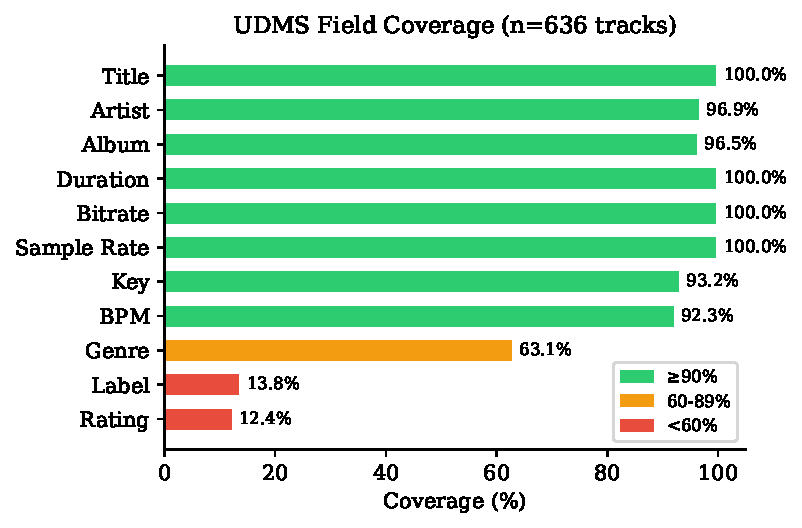
\includegraphics[width=\columnwidth]{fig_field_coverage.pdf}
  \caption{UDMS field coverage across 636 tracks. Green: $\geq$90\%; orange: 60--89\%; red: $<$60\%. Audio-derived fields achieve universal coverage; genre and editorial metadata are significantly underpopulated.}
  \label{fig:field_coverage}
\end{figure}

\subsection{Metadata Completeness Tiers}

Figure~\ref{fig:completeness} shows the distribution of tracks across completeness tiers. Only 60.2\% of tracks reach the ``Full'' tier (title + artist + BPM + key + genre), and only 1.6\% have complete metadata including label and rating. Critically, 39.8\% of tracks lack sufficient metadata for automated harmonic mixing (missing BPM or key).

\begin{figure}[t]
  \centering
  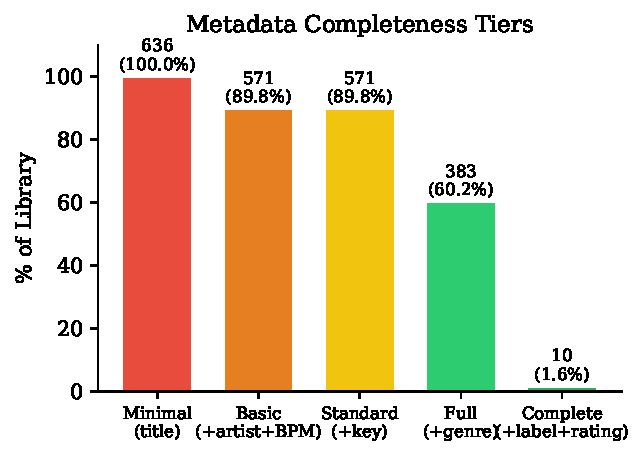
\includegraphics[width=\columnwidth]{fig_completeness_tiers.pdf}
  \caption{Metadata completeness tiers. Each tier includes all fields from previous tiers. Only 1.6\% of tracks have complete metadata including label and rating.}
  \label{fig:completeness}
\end{figure}

\subsection{BPM Distribution}

Figure~\ref{fig:bpm} shows the BPM distribution (n=587, range 73--175, mean 130.7, SD 14.5). Values cluster heavily in the 120--149 range (82.1\%), consistent with electronic dance music conventions. The 120--129 BPM bucket contains the most tracks (34.1\%), followed by 130--139 (28.1\%) and 140--149 (19.9\%). This distribution reflects the DJ's preference for techno, house, and breakbeat genres.

\begin{figure}[t]
  \centering
  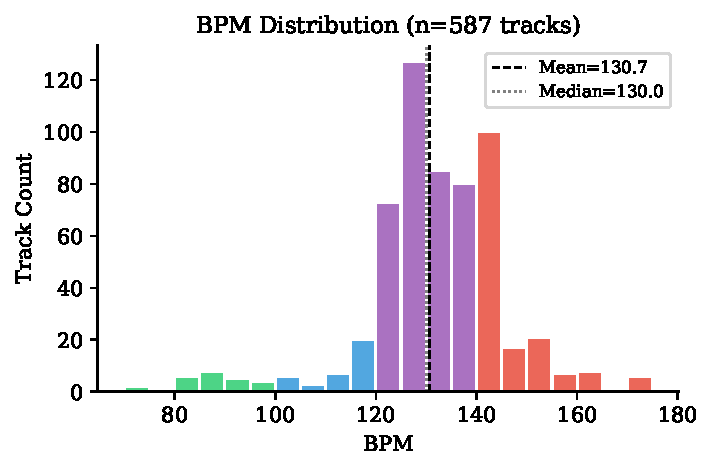
\includegraphics[width=\columnwidth]{fig_bpm_distribution.pdf}
  \caption{BPM distribution (n=587). Mean=130.7 (dashed), median=130.0 (dotted). 82.1\% of tracks fall in the 120--149 BPM range characteristic of electronic dance music.}
  \label{fig:bpm}
\end{figure}

\subsection{Musical Key Distribution}

Figure~\ref{fig:key} shows the Camelot key distribution. Of 593 keyed tracks, 88.4\% are in minor keys (Camelot ``A'') and 11.6\% in major keys (``B''). This strong minor-key bias is characteristic of electronic dance music, where minor keys convey tension and energy suited to dancefloor contexts~\citep{bernardes2018harmonic}. The most common keys are 4A (F~minor, 11.0\%), 8A (A~minor, 10.6\%), and 6A (G~minor, 10.3\%), with the three most common minor keys accounting for 31.9\% of all keyed tracks.

43 tracks (6.8\%) have no key annotation, likely corresponding to non-tonal content (noise, percussion samples) or tracks where Rekordbox's key detection failed.

\begin{figure}[t]
  \centering
  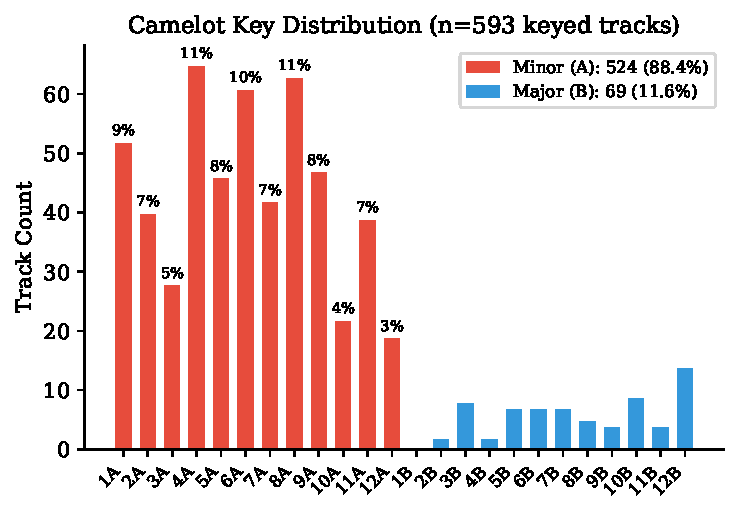
\includegraphics[width=\columnwidth]{fig_key_distribution.pdf}
  \caption{Camelot key distribution (n=593). Minor keys (red) dominate at 88.4\%, consistent with electronic dance music conventions.}
  \label{fig:key}
\end{figure}

\subsection{Per-Source Metadata Quality}

Figure~\ref{fig:source} shows metadata coverage by acquisition source. Source strongly predicts metadata quality:
\begin{itemize}
  \item \textbf{DJ Playlists} (n=269): 100\% BPM/key coverage (analyzed by Rekordbox), but only 66.9\% genre coverage and 2.6\% rating coverage.
  \item \textbf{Monthly DLs} (n=117): 100\% BPM/key, 70.1\% genre, 29.9\% ratings---but 0\% labels.
  \item \textbf{SoulSeek} (n=83): 100\% BPM/key, 72.3\% genre, 63.9\% labels---but 0\% ratings and 89.2\% artist (vs 97--100\% elsewhere).
  \item \textbf{Local/Other} (n=153): Lowest BPM/key coverage (70.6\%/71.9\%), 46.4\% genre.
\end{itemize}
This per-source variation reveals that metadata quality is not uniform across a library but depends on how tracks were acquired and curated.

\begin{figure}[t]
  \centering
  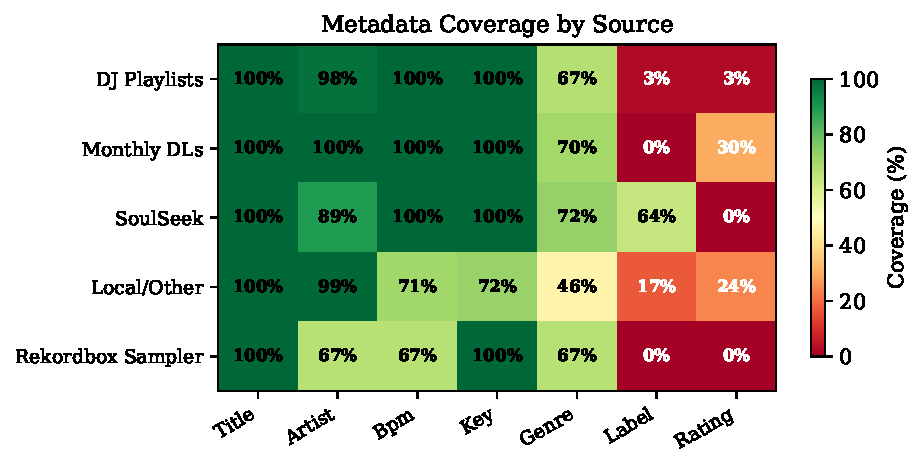
\includegraphics[width=\columnwidth]{fig_source_heatmap.pdf}
  \caption{Metadata coverage by acquisition source. Cell values show percentage of tracks with field populated. SoulSeek has the best label coverage (63.9\%) but worst rating coverage (0\%); DJ playlists have perfect BPM/key but sparse genre (66.9\%).}
  \label{fig:source}
\end{figure}

\subsection{Genre Taxonomy}

401 tracks carry genre annotation across 70 unique genre strings---a high fragmentation rate indicating inconsistent manual annotation. After grouping similar genres, the library spans: Techno (17.0\%), Breaks/Electro (14.2\%), Dub Techno (12.0\%), House (8.5\%), Dub/Dubwise (7.0\%), Psy Tech (5.7\%), Dubstep (5.2\%), UK Garage/2-Step (4.2\%), and Hardgroove (4.2\%).

The 235 untagged tracks (36.9\%) still carry title (100\%), artist (92.8\%), album (91.5\%), key (87.7\%), and BPM (85.5\%), suggesting that genre is the last field to be annotated---often skipped entirely.

\subsection{Genre Recovery via MusicBrainz}

Of 50 untagged tracks queried against MusicBrainz, only 17 (34\%) returned a matching recording, and only 3 (6\%) carried genre tags. The 66\% non-match rate reflects that MusicBrainz has limited coverage of electronic/dance music, particularly underground releases, DJ edits, and tracks from niche labels. This finding underscores that external auto-tag sources cannot reliably recover missing genre metadata in DJ libraries---the gap must be addressed through audio-based classification~\citep{choi2019zeroshot} or platform-native annotation workflows.

\section{Discussion}

\subsection{Genre as the Critical Bottleneck}

Genre annotation is the most impactful metadata gap in DJ libraries. At 63.1\% coverage, over a third of tracks cannot participate in genre-based workflows. Moreover, the 70 unique genre strings present a taxonomy problem---manual annotation is inconsistent, with tracks from the same artist or release tagged differently. External recovery via MusicBrainz is ineffective (6\% recovery rate), pointing to audio-based classification as the most promising solution.

\subsection{Source-Dependent Metadata Patterns}

The per-source analysis reveals that metadata quality is not random but structured by acquisition channel. Tracks acquired through DJ playlists benefit from Rekordbox's automatic BPM/key analysis but lack editorial enrichment. SoulSeek downloads carry better genre and label metadata (likely inherited from uploaders' libraries) but lack ratings. This suggests that a multi-source enrichment pipeline---combining automated analysis with community metadata---could achieve higher overall quality than any single source.

\subsection{Minor Key Bias}

The 88.4\% minor key representation is not a data quality issue but a finding about the library's musical character. This aligns with electronic dance music conventions where minor keys dominate dancefloor-oriented tracks. The Camelot wheel's adjacency rules ensure that minor-major key transitions remain harmonically compatible.

\subsection{Rating Sparsity}

Only 12.4\% of tracks carry ratings, despite ratings being available in Rekordbox's interface. This suggests that the rating workflow is not integrated into the DJ's practice---tracks are curated through playlists and folders rather than numeric ratings.

\subsection{Impact on Automated DJ Workflows}

We assess metadata readiness for three common DJ workflows:
\begin{itemize}
  \item \textbf{Harmonic mixing} (requires BPM + key): 84.3\% of tracks (536/636) are ready.
  \item \textbf{Genre-based playlists} (requires genre): 63.1\% of tracks are ready.
  \item \textbf{Energy-based sequencing} (requires ratings): 12.4\% of tracks are ready.
\end{itemize}
Automated DJ tools operating on real-world libraries will encounter missing metadata in 16--88\% of cases depending on the workflow.

\subsection{Limitations}

This study analyzes a single library from one DJ. Library composition reflects the DJ's personal taste (electronic/bass music focus), limiting generalizability. The 636-track dataset, while substantial, is smaller than typical commercial DJ libraries. We analyze only Rekordbox XML exports; Serato and Traktor libraries may exhibit different metadata patterns. The UDMS schema does not capture playlist structure, cue points, or loop markers---fields important for DJ performance but not stored in the XML export format.

\section{Conclusion}

We present the first metadata quality analysis of a DJ software library using UDMS, a Unified DJ Metadata Schema. Our analysis of 636 tracks from a Rekordbox~7.2.8 export reveals that while audio-derived fields and musical key achieve high coverage (93--100\%), genre annotation---the field most critical for automated playlist generation---is incomplete for 36.9\% of tracks. Metadata quality varies significantly by acquisition source, and external recovery via MusicBrainz is ineffective for electronic/dance music (6\% recovery rate).

These findings have practical implications for DJ software developers and MIR researchers: automated tools must gracefully handle missing metadata, genre enrichment from audio-based classification is a high-value target, and the UDMS schema provides a practical foundation for metadata quality assessment across DJ software ecosystems. The UDMS schema and analysis tools are released as open-source at \url{https://github.com/interfluve-wav/dj-metadata-paper}.

\section{Reproducibility}

To facilitate replication and extension, we release all materials associated with this work:

\begin{itemize}
  \item \textbf{UDMS Schema and Python Implementation:} \url{https://github.com/interfluve-wav/dj-metadata-paper}
  \item \textbf{Dataset:} The 636-track Rekordbox XML export (anonymized) is included in the repository at \path{data/}. Track filenames and paths are anonymized; metadata fields are preserved.
  \item \textbf{Analysis Scripts:} \path{code/schema/udms_schema.py} contains the UDMS schema and adapters; \path{code/analyze.py} contains the analysis pipeline used to generate all figures and statistics.
  \item \textbf{Figures:} All figures are generated programmatically from the dataset; source scripts are in \path{code/}.
  \item \textbf{License:} MIT License.
\end{itemize}

ISMIR 2026 requires code availability for reproducibility. The repository is public and will be archived with a Zenodo DOI prior to submission.

\section*{Acknowledgments}

[Anonymized for review.]

\bibliography{references}

\section{AI Usage Statement}
AI tools were used in the research and writing process for code generation, literature search, and text editing assistance.

\section{Ethics Statement}
This study analyzes a single DJ's personal music library. No human subjects were involved; all metadata was self-generated through normal software use. The dataset contains no personally identifiable information beyond file paths, which are anonymized in the released data.

\end{document}
